\documentclass{article}
\usepackage[dutch]{babel}
\usepackage{hyperref}
\usepackage{graphicx}
\usepackage[bottom=2.5cm, right=2.5cm, left=2.5cm, top=2.5cm]{geometry}

\title{Startvergadering ML sessie 5}
\author{Team $\exists$uler: \textit{Daan, Marie, Zeineb, Florian, Vincent, Jasper, Lasha, Younes}}
\date{Vrijdag 10 november 2023}

\begin{document}
	
	\maketitle
	
	\section*{Vooraf}
	
	Deze sessie zijn we met 1 teamlid minder. Vincent is afwezig vanwege de begrafenis van zijn grootvader. Hij bracht reeds een aantal zaken in orde voor de aanvang van deze sessie:
	
	\begin{itemize}
		\item Er werd op OneDrive een map \textit{Implementatie} aangemaakt met daarin de bijhorende bestanden \texttt{procedures.py}, \texttt{simulaties.ipynb} en tot slot ook \texttt{voorbeelden.ipynb}. Elk bestand werd ook voorzien van een stukje commentaar met duidelijke instructies over hun gebruik, zoals te zien is in figuur \ref{fig:bestanden}.
		\item In de KanBan werd een nieuw tabblad \textit{Implementatie} aangemaakt, voorzien van een tabel waarin alles kan ingevuld worden, analoog aan het tabblad \textit{Oefeningen}. Dit is te zien in figuur \ref{fig:kanban}.
		\item De procedures \texttt{xsample}, \texttt{ysample}, \texttt{ols}, \texttt{knn} en \texttt{mls} werden al volledig geprogrammeerd in \texttt{procedures.py} en volledig voorzien van voorbeelden in \texttt{voorbeelden.ipynb}. Ook werd simulatie 1 al helemaal afgewerkt.
	\end{itemize}
	
	\begin{figure}
		\centering
		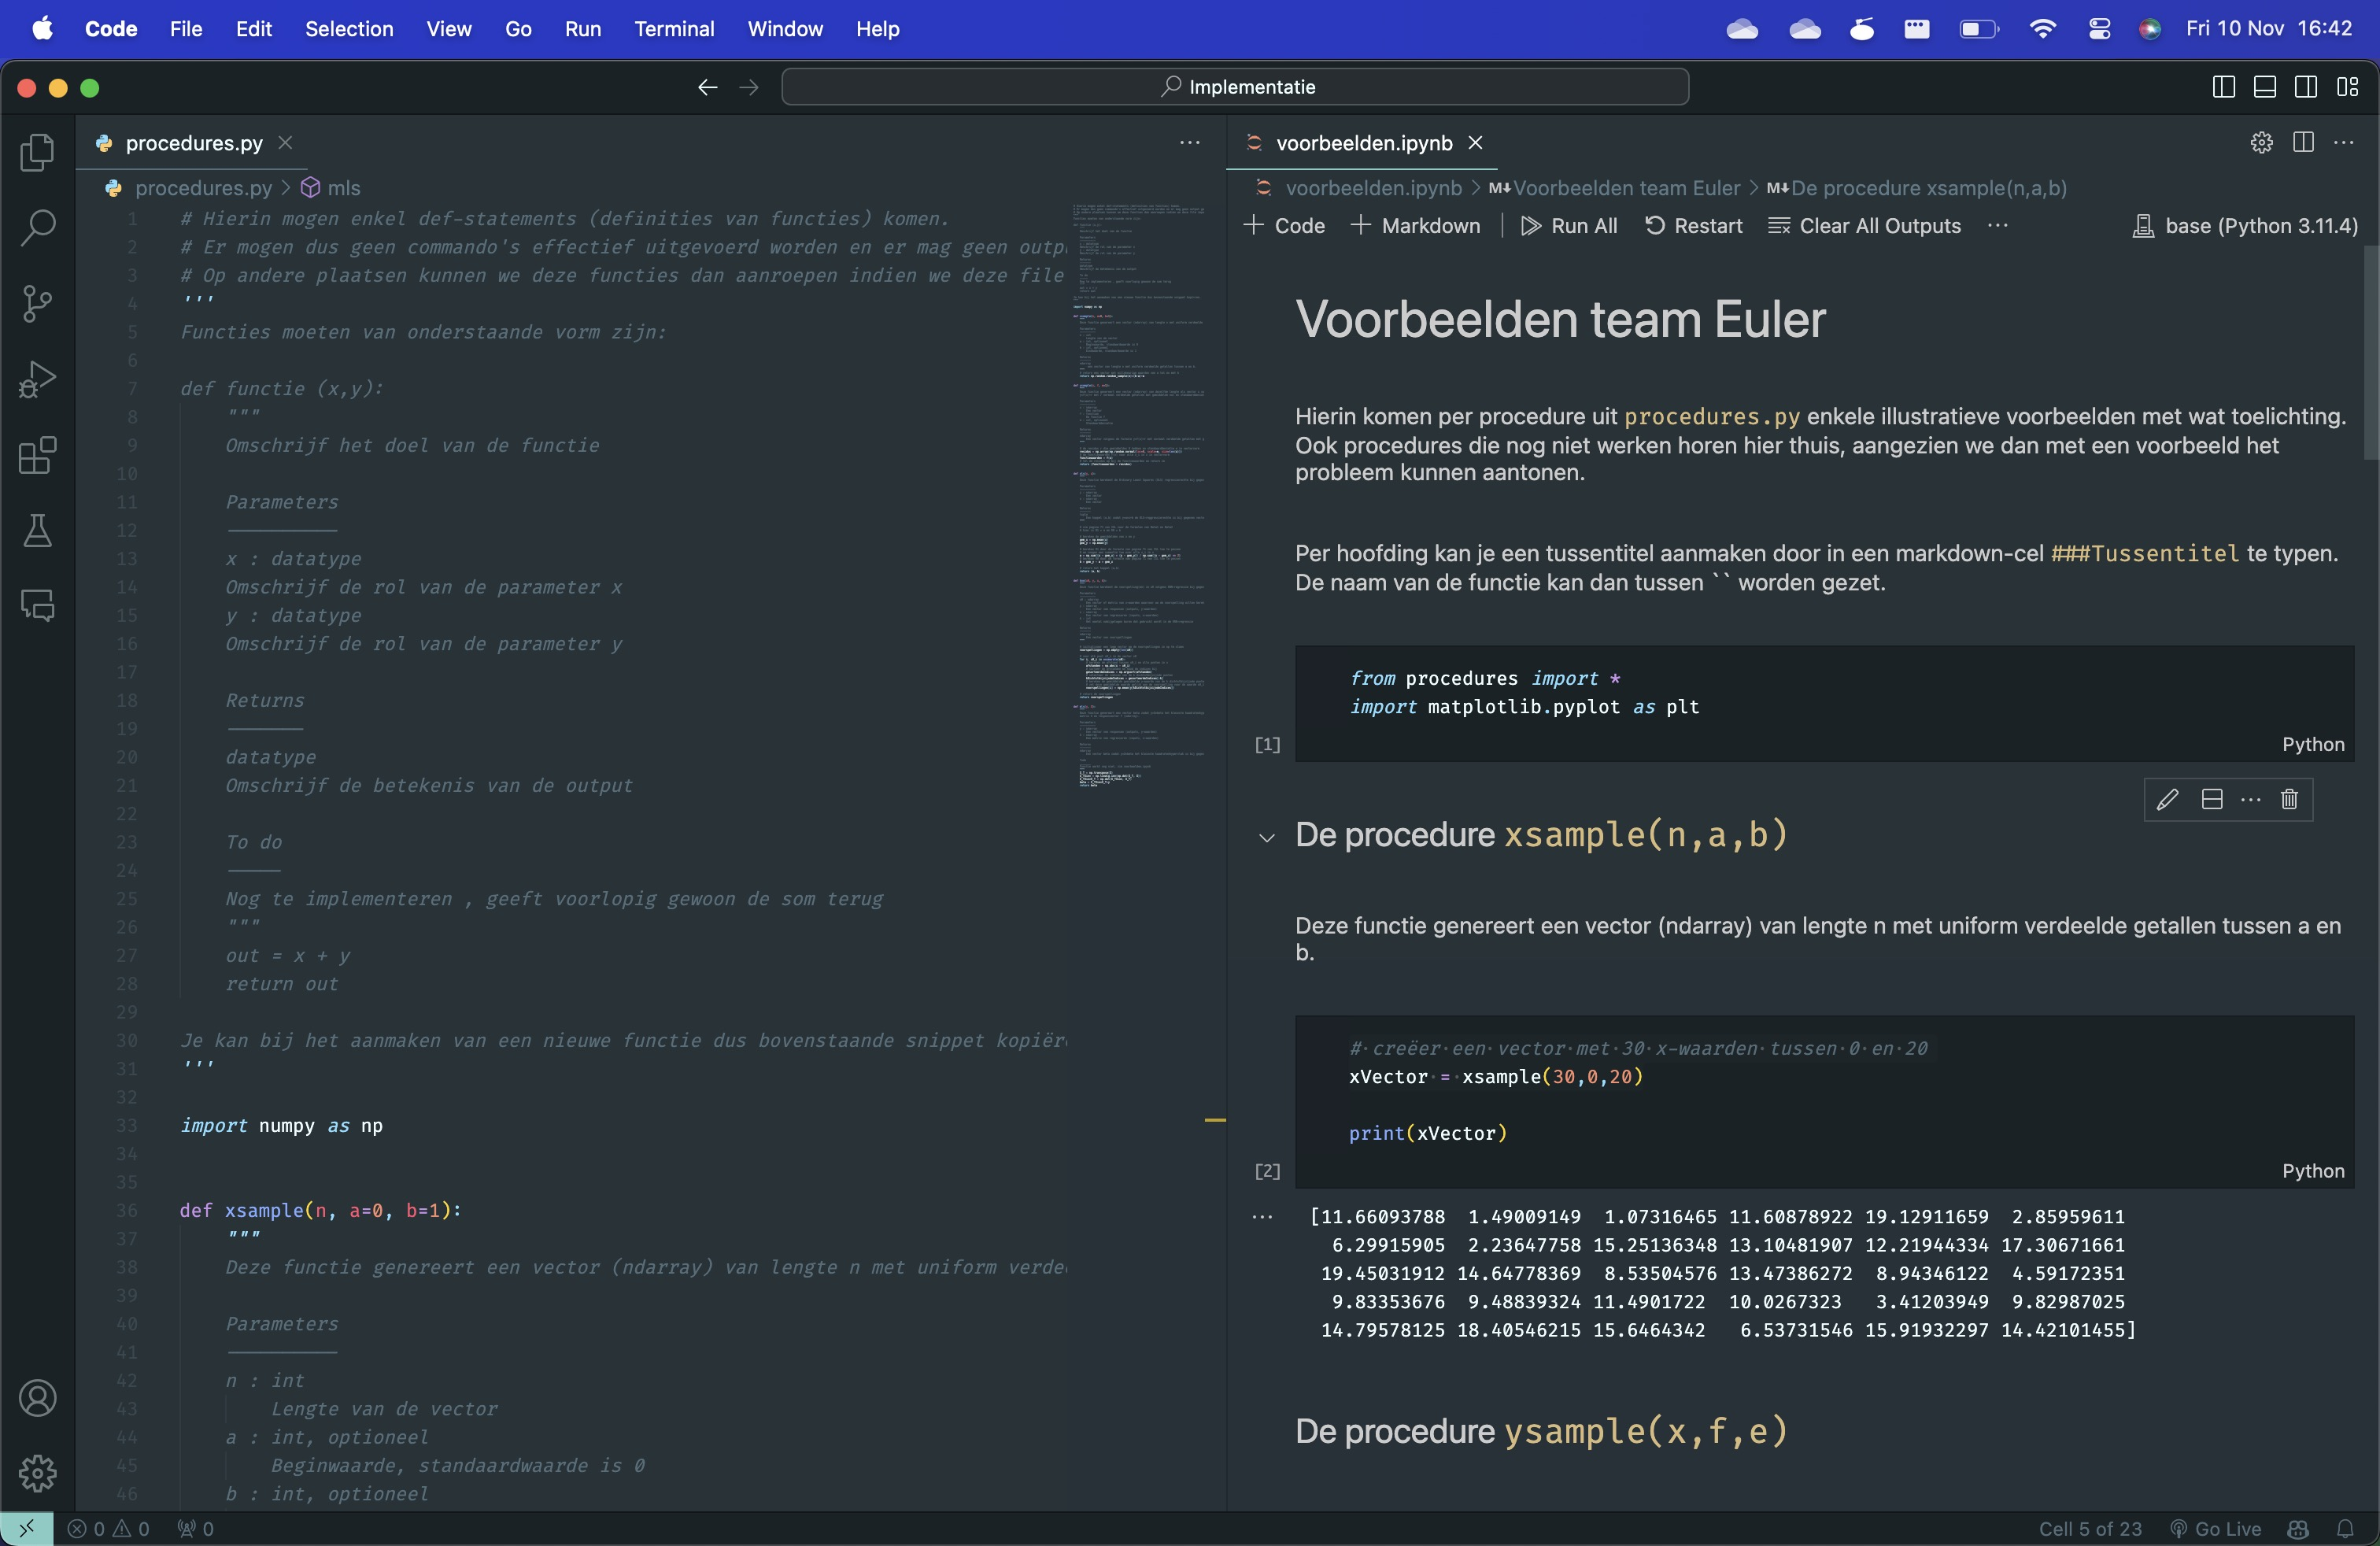
\includegraphics[width=0.9\textwidth]{bestanden}
		\caption{De bestanden \texttt{procedures.py} (links) en \texttt{voorbeelden.ipynb} (rechts), elk voorzien van commentaar met duidelijke instructies.}
		\label{fig:bestanden}
	\end{figure}
	
	\begin{figure}
		\centering
		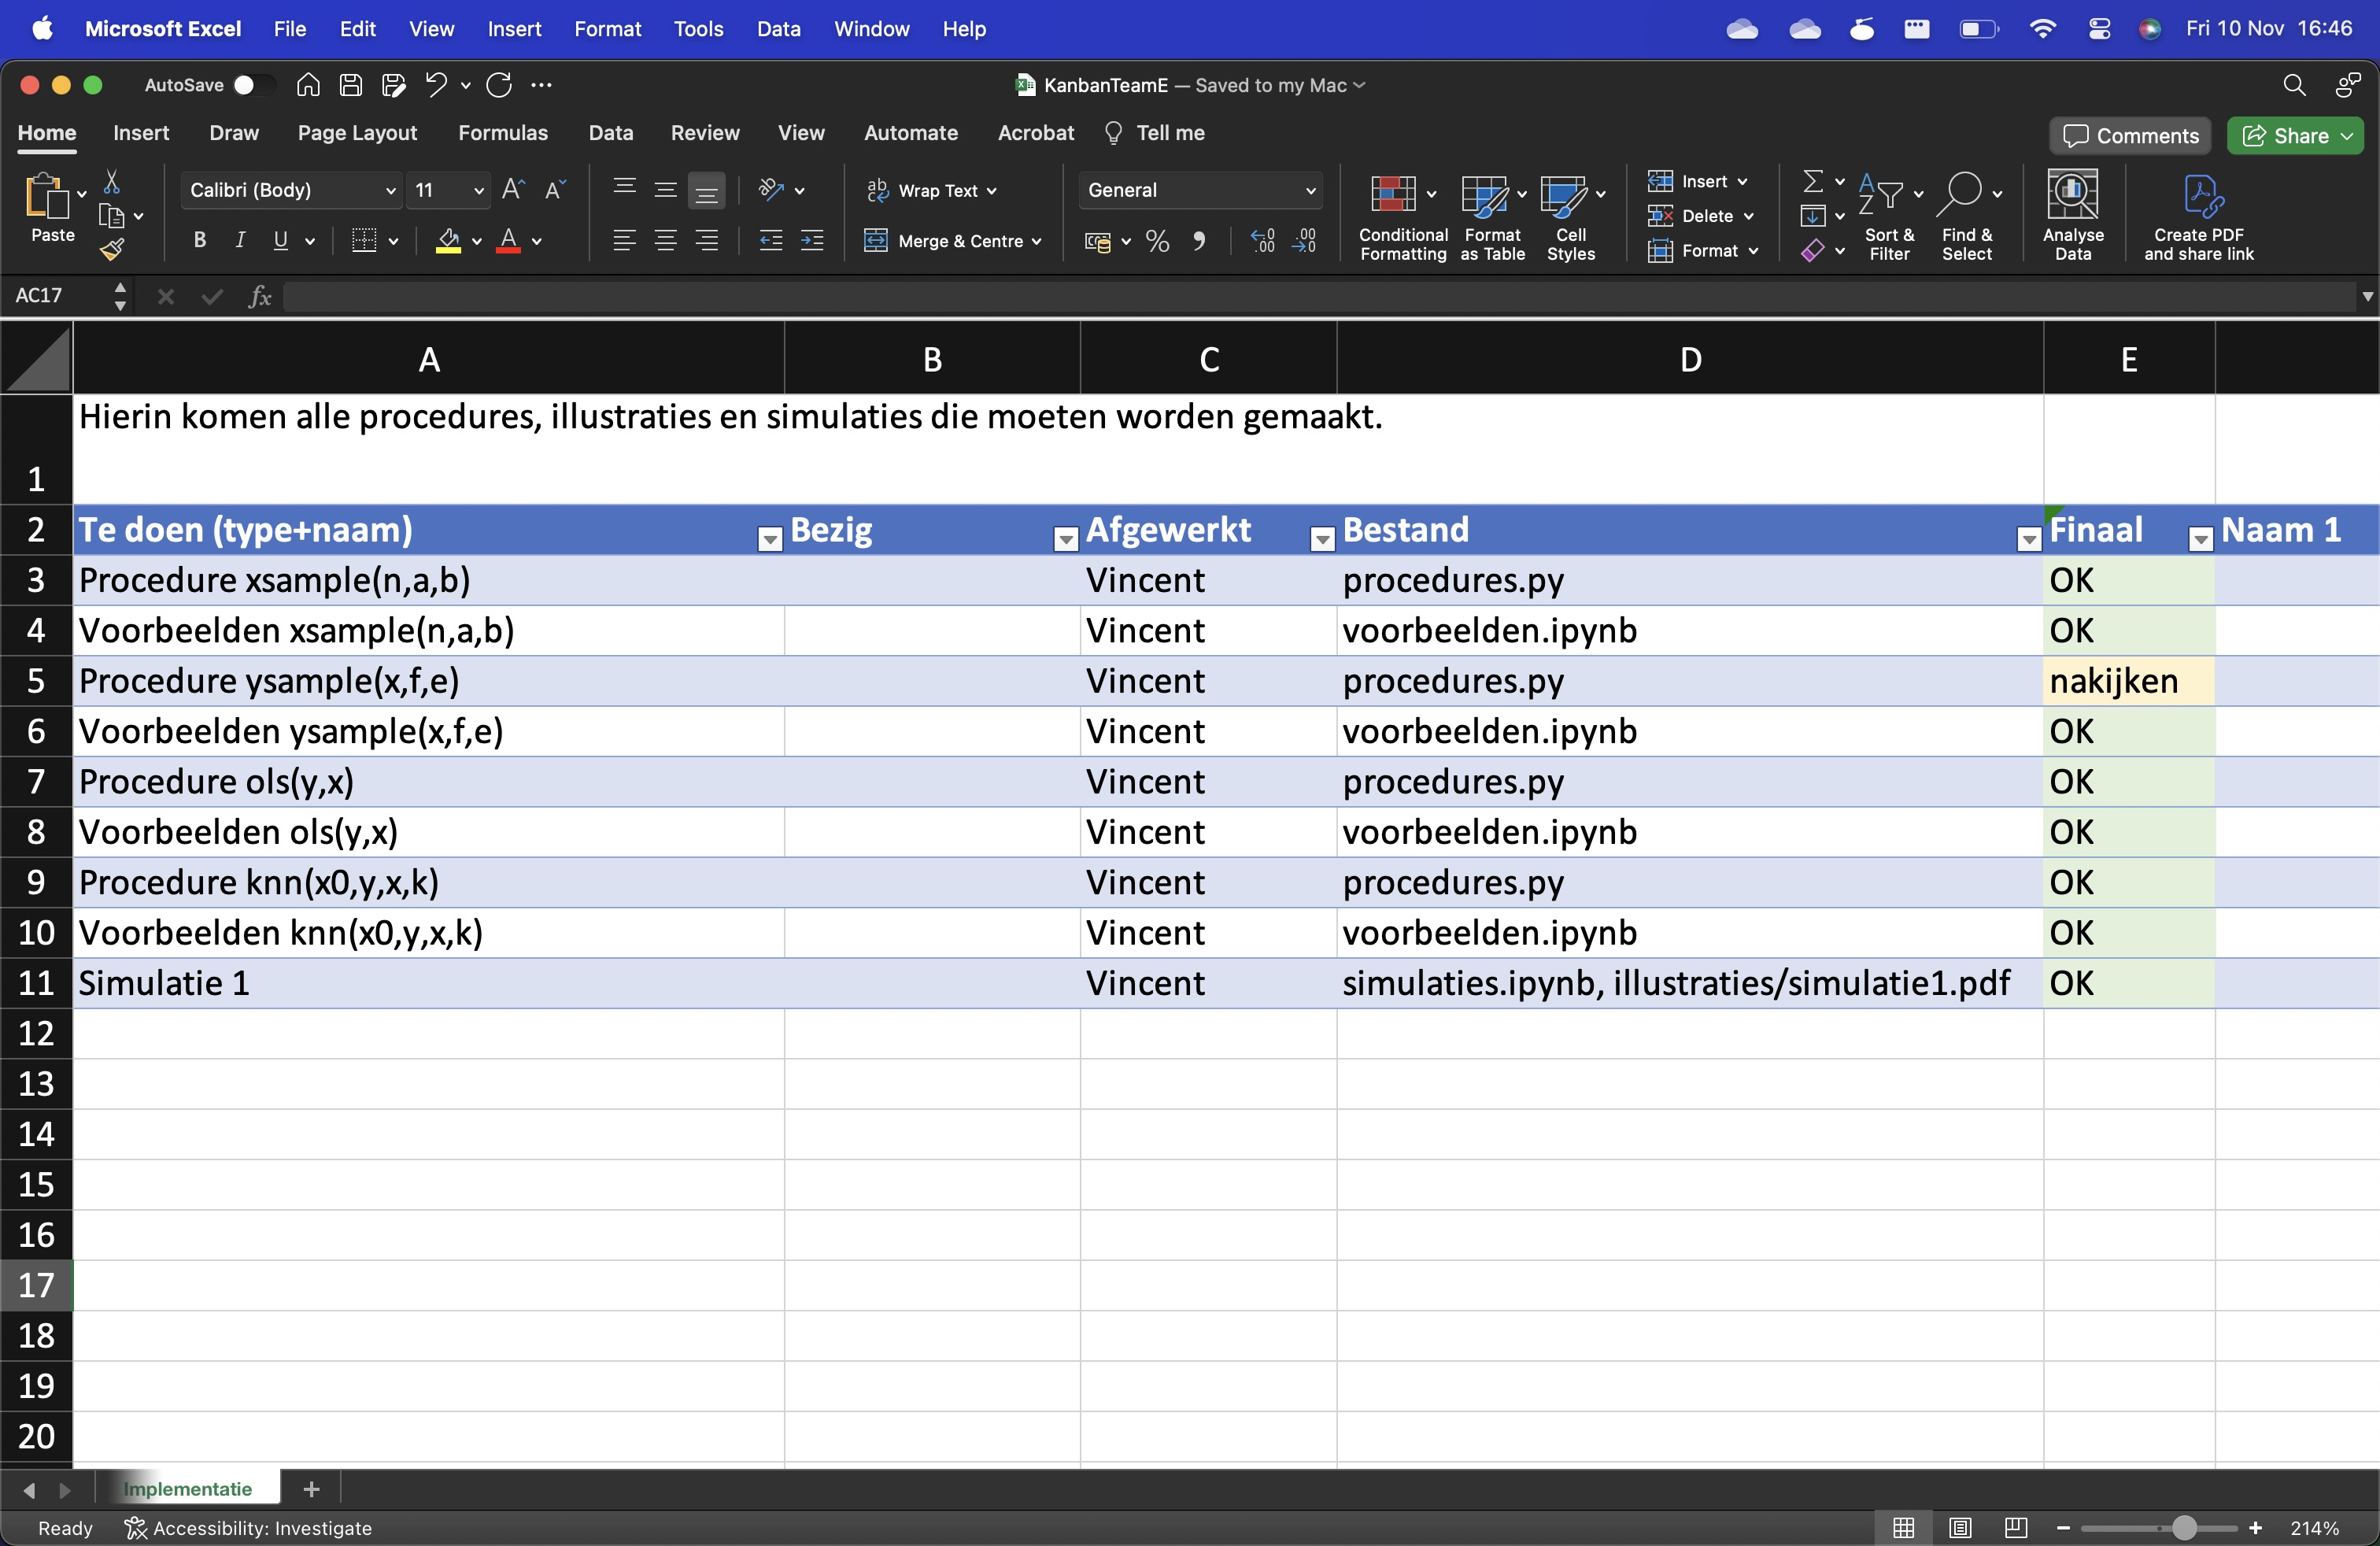
\includegraphics[width=0.9\textwidth]{kanban}
		\caption{Het nieuw aangemaakte tabblad \textit{Implementatie} in de KanBan met daarin alle taken die Vincent reeds afwerkte vóór de aanvang van de sessie.}
		\label{fig:kanban}
	\end{figure}
	
	\section*{Stand van zaken oefeningen}

	De afgelopen twee weken hebben we zo veel mogelijk oefeningen afgewerkt. Na het herlezen van \texttt{MLsessie03.pdf}, stelde Vincent vast dat onze oefeningen niet de juiste naamgeving hadden. Dit werd dan ook meteen aangepast, zodat het nu wel correct is. Florian zal nog een oefening afwerken en er moeten zo snel mogelijk nog een paar oefeningen nagekeken worden.
	
	\section*{Takenverdeling}
	
	Het grootste deel van het team zal de basismethodes, waar Vincent aan begonnen is, verder implementeren en starten met de vergelijking met de ingebouwde procedures uit \texttt{sklearn}. De teamleden die dit zullen doen zijn Lasha, Zeineb, Marie, Florian en Daan.
	
	Jasper en Younes zullen werken aan de implementatie van de bijkomende toepassing, namelijk \textit{Support Vector Machines}.
	

\end{document}